%\documentclass[pdf,final,colorBG,slideColor]{prosper}
\documentclass[xcolor=dvipsnames]{beamer}
%%\usetheme{default}
\usecolortheme[named=Maroon]{structure}
%\usetheme{Boadilla}
\usetheme{Madrid}
\useoutertheme{default}%[footline=empty]{infolines}

% \usepackage{helvet}
% \usepackage{enumerate}
% \usepackage{amsmath}
% \usepackage{amsfonts}
% \usepackage{graphicx}
% \usepackage{ulem}
% \usepackage{multirow}
\usepackage{comment}
\usepackage{xspace}
%\usepackage{columns}

\usepackage[absolute,overlay]{textpos}
\usepackage[ruled,linesnumbered]{./algorithm2e}
%%for algorithm2e package, label has to be following caption in the same line!!!
\renewcommand{\algorithmcfname}{ALGORITHM}
\SetAlFnt{\small}
\SetAlCapFnt{\small}
\SetAlCapNameFnt{\small}
\SetAlCapHSkip{0pt}
\IncMargin{-\parindent}

%\RequirePackage{algorithmic}
%\RequirePackage{algorithm}
% \renewcommand{\algorithmicrequire}{\textbf{Inputs:}}
% \renewcommand{\algorithmicensure}{\textbf{Outputs:}}


%\newtheorem{theorem}{Theorem}
%\newtheorem{lemma}{lemma}
%\newtheorem{corollary}{Corollary}
%\newtheorem{proposition}{Proposition}
%\newtheorem{Q}{Question}
%\newtheorem{Exa}{Example}
%\newtheorem{Definition}{Definition}


\newcommand{\Fq}{{\mathbb{F}}_{q}}
\newcommand{\Fkk}{{\mathbb{F}}_{2^k}}
\newcommand{\Zkk}{{\mathbb{Z}}_{2^k}}
\newcommand{\Fkkx}[1][x]{\ensuremath{\mathbb{F}}_{2^k}[#1]\xspace}
\newcommand{\Grobner}{Gr\"{o}bner\xspace}
%\newcommand{\Grobner}{Gr\"{o}bner}
\newcommand{\bi}{\begin{itemize}}
\newcommand{\ei}{\end{itemize}}
\newcommand{\F}{{\mathcal{F}}}
\newcommand{\B}{{\mathbb{B}}}


\title[Presentation]{Formal Verification of Sequential Galois Field Arithmetic Circuits using Algebraic Geometry}

\author[Xiaojun Sun]{{\bf Xiaojun Sun}$^1$, Priyank Kalla$^1$, Tim Pruss$^1$, Florian Enescu$^2$}

%\email{rostamian@umbc.edu}
\institute[Univ. of Utah]{
%\includegraphics[height=17mm]{/Users/Kalla/teaching/Comp-Algebra-Course/lectures/old_ulogo.eps}\\
$^1$Electrical and Computer Engineering, University of Utah, Salt Lake City, USA\\
$^2$Mathematics \& Statistics, Georgia State University, Atlanta, USA\\
\ \\
\{{\bf xiaojuns}, kalla, tpruss\}@ece.utah.edu, fenescu@gsu.edu\\
\ \\
\ \\
{\bf Session 12.2 -- Long Presentation}\\
}


\date{}
%\slideCaption{}

%% Images
%\pgfdeclareimage[width=.4in]{fg:logo}{/Users/Kalla/teaching/Comp-Algebra-Course/lectures/old_ulogo.eps} 

%%%%%%%%%%%%%%%%%%%%%%%%%%%%%%%%%%%%%%%%%%%%%%%%%%
%%%%%%%%%%%%%%%%%%%%%%%%%%%%%%%%%%%%%%%%%%%%%%%%%%
%%%%%%%%%%%%%%%%%%%%%%%%%%%%%%%%%%%%%%%%%%%%%%%%%%
\begin{document}


%----------- titlepage ----------------------------------------------%
\begin{frame}[plain]
  \titlepage

\end{frame}

%\maketitle
%%%%%%%%%%%%%%%%%%%%%%%%%%%%%%%%%%%%%%%%%%%%%%%%%%
\begin{frame}{\large{Motivation and Basic Idea}}
\bi
\item Target problems
	\bi
	\item Given:
		\bi
		\item  A Galois field (GF) and normal basis representation
		\item A word level specification polynomial
		\item A sequential implementation of polynomial computation
		\ei
	\item Aim: perform property checking on the sequential implementation
	\ei
\item Focus
	\bi
	\item Analyze and abstract the function of sequential GF arithmetic circuits
	\item Implicit \alert{word-level} finite state machine (FSM) traversal
	\ei
\item Motivation
	\bi
	\item Data flow $=$ word level info
	\item Conventional techniques are bit-level
	\item Gr\"obner basis theory can assist bit-to-word conversion
	\item Word level $\to$ implicit $\to$ efficient!
	\ei
\ei
\end{frame}
%%%%%%%%%%%%%%%%%%%%%%%%%%%%%%%%%%%%%%%%%%%%%%%%%%
\begin{frame}{\large{Outline}}
\bi
\item Background application
\item Preliminaries
	\bi
	\item Field, polynomial ideal
	\item Abstraction using Gr\"obner basis
	\item Normal basis representation
	\ei
\item Methodology
	\bi
	\item Basic algorithm
	\item Improving our approach
	\ei
\item Experiment results
\item Conclusion
\ei
\end{frame}
%%%%%%%%%%%%%%%%%%%%%%%%%%%%%%%%%%%%%%%%%%%%%%%%%%
\begin{frame}{\large{Background}}
\bi
\item Cryptography: polynomial computation over $\Fkk$
	\bi
	\item Algebraic nature (GF) of the computation (polynomial)
	\item Datapath size $k$: very large
	\ei
\vspace{5mm}
\item Verification of sequential circuits is needed
	\bi
	\item Verify sequential GF circuits designed using normal basis
	\item Complicated circuits need to be verified
	\item Sequential circuits bounded by $k$ clock cycles
	\item Example: [Reyhani-Masoleh and Hasan, \textit{“Sequential normal basis multipliers”}, Trans on Computer, 2005]
	\ei
\ei
\end{frame}
%%%%%%%%%%%%%%%%%%%%%%%%%%%%%%%%%%%%%%%%%%%%%%%%%%%



\begin{frame}{\large{Our approach vs Conventional approach}}
\vspace{-0.1in}
\begin{figure}[H]
\centering{
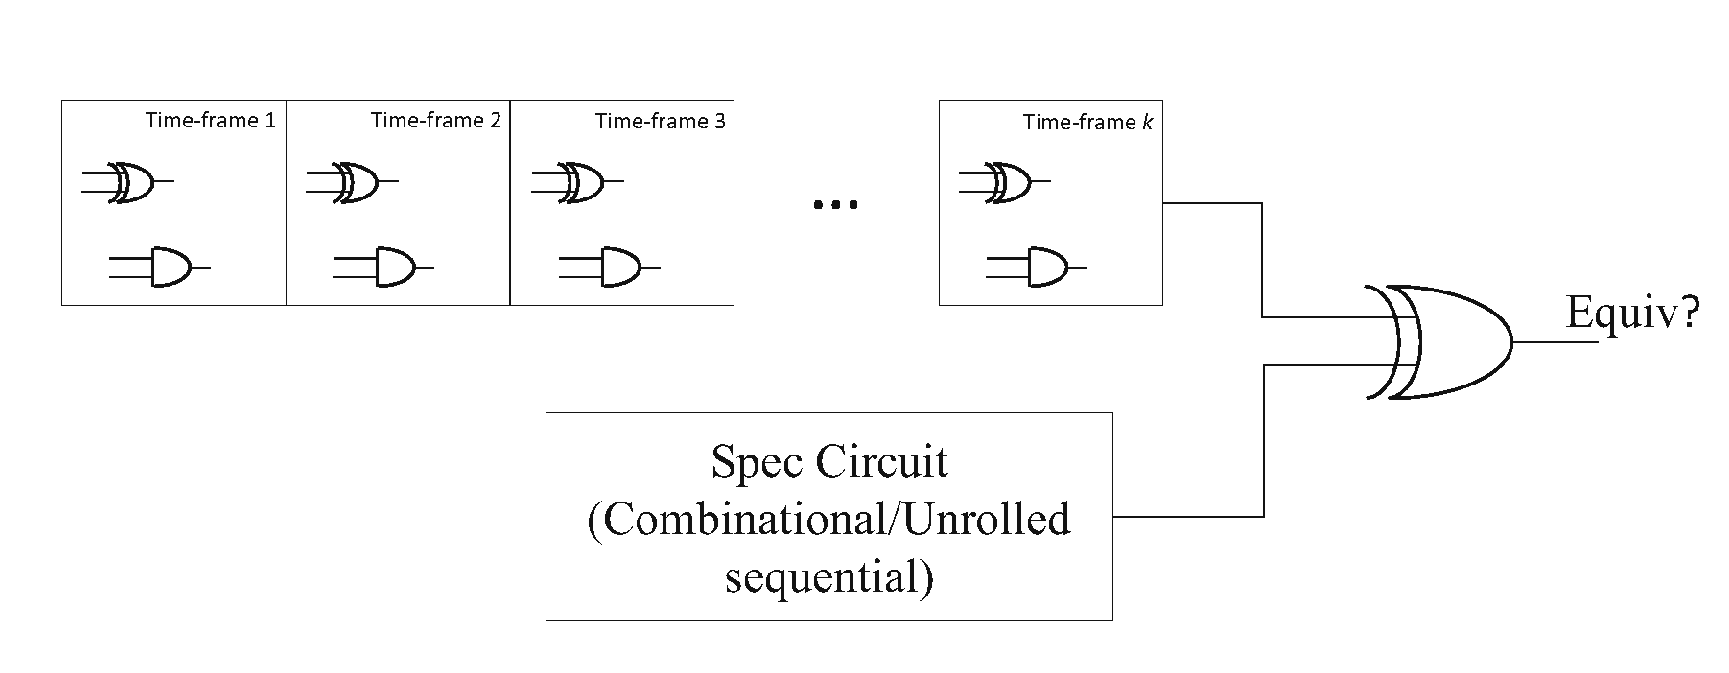
\includegraphics[width=4.5in]{./convention.eps}
}
\end{figure}
\vspace{-0.4in}
\bi
\item Conventional: explicitly unroll $k$ time-frames
	\bi
	\item Bit-blasting!
	\ei
\item New: \alert{Implicitly} unroll the finite state machine (FSM)
	\bi
	\item Update the spec poly for $k$ times ($R = \F(A,B)$) when unrolling
	\item $R_1 = \F(A_{init},B_{init}),~R_2 = \F(A_{1},B_{1}) = \F^2(A_{init},B_{init}),~ 
	\cdots, ~ R_k = \F^k(A_{init},B_{init}) = A_{init}\cdot B_{init}$
	\ei
\ei
\end{frame}
%%%%%%%%%%%%%%%%%%%%%%%%%%%%%%%%%%%%%%%%%%%%%%%%%%%%%%%%%
%%%%%%%%%%%%%%%%%%%%%%%%%%%%%%%%%%%%%%%%%%%%%%%%%%%%%%%%%%%%
\begin{frame}{\large{Illustration of implicit unrolling}}
\vspace{-0.1in}
\begin{figure}[hbt]
\centering{
%\begin{minipage}{12cm}
\includegraphics[width=4.5in]{./Moore.eps}
% \vspace{-0.2in}
%\caption{A simple Moore FSM and its state transition graph}
%\end{minipage}
\label{fig:Moore}}
\end{figure}
\vspace{-0.2in}
\bi
\item Model: restricted Moore finite state machine
	\bi
	\item Some sequential arithmetic circuits will give results after running for $k$ clock cycles
	\item The initial operands are preloaded in register files
	\ei
\item State transitions on this model:
$$R_{k} = Tr(R_{k-1}) = Tr(Tr(\cdots Tr(R_{init})\cdots)) = Tr^k(R_{init})$$
\ei
\end{frame}
%%%%%%%%%%%%%%%%%%%%%%%%%%%%%%%%%%%%%%%%%%%%%%%%%%%
\begin{frame}{\large {Galois Field Overview}}
%\vspace{-0.2in}
%\ptsize{10}
\textbf {Galois field}(GF) $\mathbb{F}_q$ is a finite field with $q$
elements, $q = p^k$
\begin{itemize}
\item Commutative Ring with unity, associate, distributive laws
\item Closure property: $+,-,\times$, inverse ($\div$)
\end{itemize}


Our interest: $\mathbb{F}_{q} = \mathbb{F}_{2^k}$, i.e. $q = 2^k$
\begin{itemize}
\item  $\mathbb{F}_{2^k}$: $k$-dimensional extension of  $\mathbb{F}_{2}$
	\begin{itemize}
	\item $k$-bit bit-vector, AND/XOR arithmetic
	\end{itemize}
\end{itemize}

To construct $\mathbb{F}_{2^k}$
\begin{itemize}
\item $\mathbb{F}_{2^k} \equiv \mathbb{F}_{2}[x] \pmod {P(x)}$
\item $P(x) \in \mathbb{F}_{2}[x]$, irreducible polynomial of degree $k$
\item $P(\alpha)=0,\ \alpha = $Primitive element
\end{itemize}

\end{frame}
%%%%%%%%%%%%%%%%%%%%%%%%%%%%%%%%%%%%%%%%%%%%%%%%%%
\begin{frame}{\large{Normal basis representation for sequential circuits}}
\vspace{-0.5cm}
\bi
\item Normal basis representation: $A(a_0,\dots,a_{k-1}) = \sum_{i=0}^{k-1}a_{n(i)}\beta^{2^i}$
\item Normal element: $\beta = \alpha^t$
\item Squaring of elements represented in
normal bases can be implemented simply by a cyclic right-shift
operation.
\ei

\begin{Example}
\label{ex:nb_sq}
For $a, b \in \Fkk, (a+b)^2 = a^2 + b^2$. Applying this rule for
element squaring: 
\begin{align}
B = & b_0\beta + b_1\beta^2 + b_2\beta^4 + \dots + b_{k-1}\beta^{2^{k-1}} \nonumber\\
B^2 = &b_0^2\beta^2 + b_1^2\beta^4 + b_2^2\beta^8 + \dots + b_{k-1}^2\beta^{2^k} \nonumber\\
= &b_{k-1}\beta + b_0\beta^2 + b_1\beta^4 + \dots + b_{k-2}\beta^{2^{k-1}} \nonumber
\end{align}
as $\beta^{2^k} = \beta$ by applying Fermat's little theorem to $\Fkk$, and $b_i^2 = b_i$. 
It is an 1-bit cyclic right-shift $\to$ implemented efficiently with sequential circuit
\end{Example}
\end{frame}
%%%%%%%%%%%%%%%%%%%%%%%%%%%%%%%%%%%%%%%%%%%%%%%%%%%%%%%%%%%%%%
\begin{frame}{\large{Verification of a sequential GF multiplier (Normal basis)}}
SPEC: $R = A_{init}\cdot B_{init} \pmod {P(\alpha)}$ after $k$ clock cycles
\hspace{-0.3in}\begin{figure}[hbt]
\centering{
%\begin{minipage}{12cm}
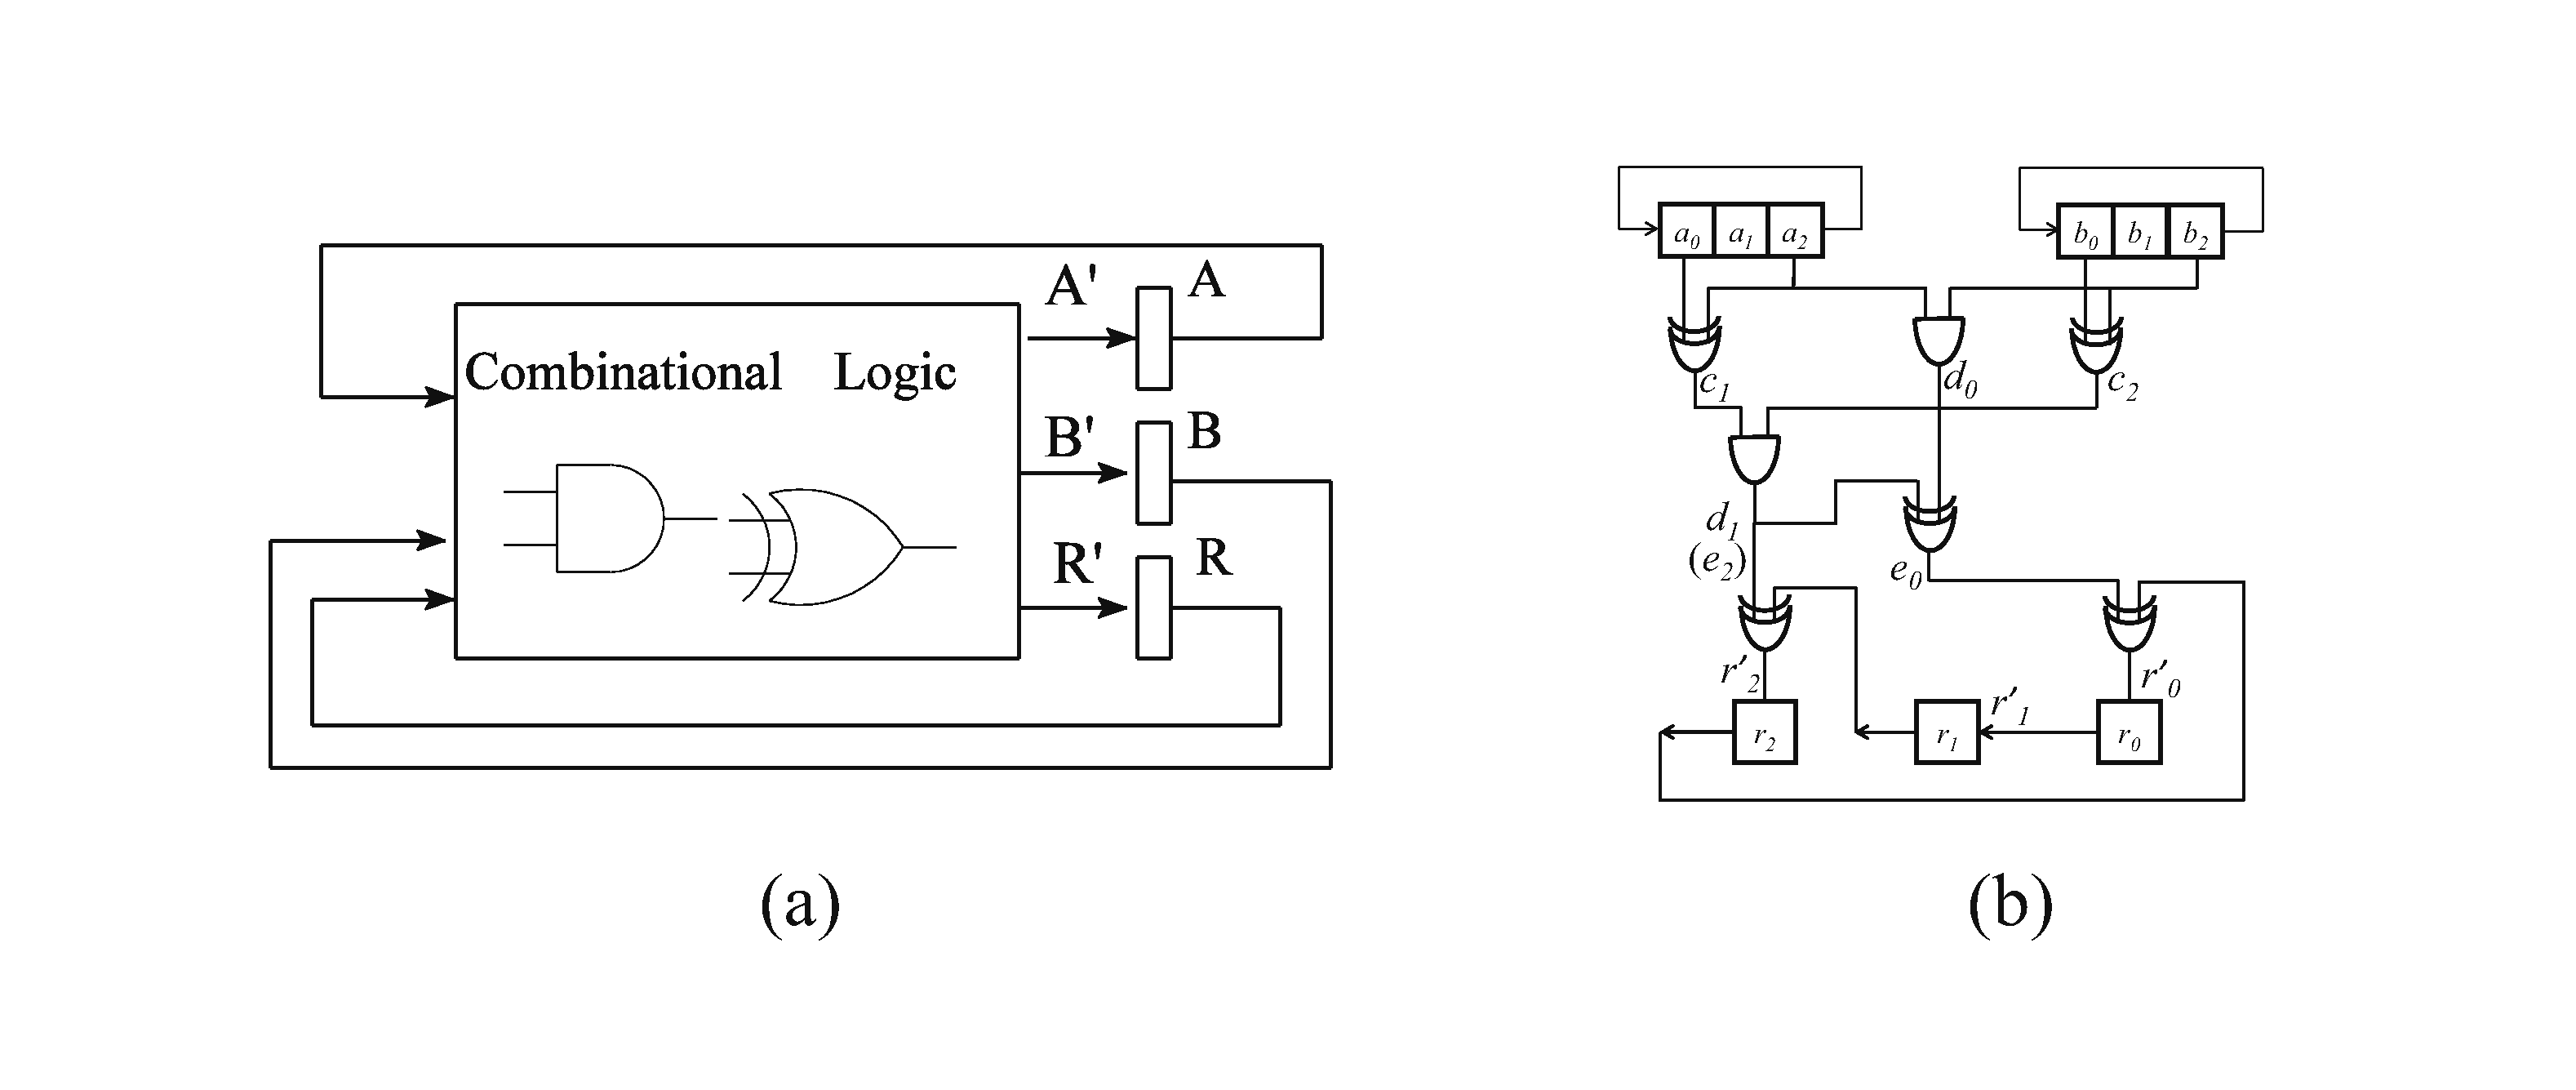
\includegraphics[width=5.5in]{./new_multi.eps}
% \vspace{-0.2in}
\caption{A 3-bit RH-SMPO and its Moore FSM model}
%\end{minipage}
\label{fig:RHmulti}}
\end{figure}
\end{frame}
%%%%%%%%%%%%%%%%%%%%%%%%%%%%%%%%%%%%%%%%%%%%%%%%%%
%\begin{comment}


%%%%%%%%%%%%%%%%%%%%%%%%%%%%%%%%%%%%%%%%%%%%%%%%%%%%%%%%%%%%%%%%

\begin{frame}{\large{Algebraic Geometry Terminology}}
\vspace{-0.2in}
%\ptsize{10}
Let $\mathbb{F}_q = GF(2^k)$:
\begin{itemize}
\item $\mathbb{F}_q[x_1, \ldots, x_n]$: ring of all polynomials with
  coefficients in $\mathbb{F}_q$ 
\item Given a set of polynomials:
\begin{itemize}
\item $f, f_1, f_2, \dots , f_s \in \mathbb{F}_q[x_1, \dots, x_n]$
\item Find solutions to $f_1 = f_2 = \dots = f_s = 0$
\end{itemize}
\item \alert{Variety:} Set of ALL solutions to a given system of polynomial equations: $V(f_1, \dots, f_s)$
	\begin{itemize}
	\item In $\mathbb{R}\left[x,y\right]$, $V(x^2+y^2-1)=\{all\  points\  on\ circle: x^2+y^2-1=0\}$
	\item In $\mathbb{R}[x]$, $V(x^2+1)=\emptyset$
	\item In $\mathbb{C}[x]$, $V(x^2+1)=\{(\pm i)\}$
	\end{itemize}
\item Variety depends on the \alert{ideal} generated by the polynomials.
\item Reason about the Variety by analyzing the Ideals
\end{itemize}


\end{frame}
%%%%%%%%%%%%%%%%%%%%%%%%%%%%%%%%%%%%%%%%%%%%%%%%%%
%%%%%%%%%%%%%%%%%%%%%%%%%%%%%%%%%%%%%%%%%%%%%%%%%%

\begin{frame}{\large {Ideals and \Grobner basis (GB)}}
\vspace{-0.1in}


\begin{Definition}
{\bf Ideals of Polynomials:} Let $f_1, f_2, \ldots, f_s \in
\mathbb{F}_q[x_1, \dots, x_d]$. Let 
\begin{eqnarray}
J = \langle f_1, f_2 \ldots, f_s\rangle = \{f_1 h_1 + f_2 h_2 + \dots + f_s h_s:h_i\in\mathbb{F}_q[x_1, \dots, x_d]\} \nonumber 
\end{eqnarray}

$J = \langle f_1, f_2 \ldots, f_s\rangle$ is an ideal generated by
$f_1, \ldots, f_s$ and the polynomials are called the generators. 
\end{Definition}

\vspace{-0.1in}
%\ptsize{10}

\begin{itemize}
\item Different generators can generate the same ideal
\item $\langle f_1,\cdots,f_s \rangle=\cdots=\langle g_1,\cdots,g_t
  \rangle$
\item Some generators are a ``better'' representation of the ideal
\item A (reduced){\bf Gr\"obner basis} is a ``canonical'' representation of an ideal
\end{itemize}

Given $F = \{f_1, f_2,\cdots, f_s\}$, Compute a GB (using Buchberger's algorithm) $G =
\{g_1,g_2,\cdots,g_t\}$, such that $I = \langle F \rangle = \langle G \rangle$

\begin{center}
$V(F)=V(G)$
\end{center}
\end{frame}

%%%%%%%%%%%%%%%%%%%%%%%%%%%%%%%%%%%%%%%%%%%%%%%%%%



%%%%%%%%%%%%%%%%%%%%%%%%%%%%%%%%%%%%%%%%%%%%%%%%%%

\begin{frame}{\large {Use of Elimination Term Ordering}}
%\ptsize{10}
\begin{itemize}
\item GB computation requires a term order
\item Let ideal $I = \langle f_1, f_2, f_3 \rangle$ where
	\begin{itemize}
	\item $f_1 = x^2 + y + z - 1$
	\item $f_2 = x + y^2 + z - 1$
	\item $f_3 = x + y + z^2 - 1$
	\end{itemize}
\item The \Grobner basis of $I$ with lex order $(x > y > z)$ is
	\begin{itemize}
	\item $g_1 = x + y + z^2 - 1$
	\item $g_2 = y^2 - y - z^2 + z$
	\item $g_3 = 2yz^2 + z^4 - z^2$
	\item $g_4 = z^6 - 4z^4 + 4z^3 - z^2$
	\end{itemize}
\item $g_2,g_3$ and $g_4$: only contain variables $y$ and $z$
	\begin{itemize}
	\item Eliminates variable $x~\Leftrightarrow  ~\exists_x$ in Boolean formula!
	\end{itemize}
\item $g_4$: only contains the variable $z$ $\to$ eliminates $x$ and $y$
\end{itemize}
\end{frame}

%%%%%%%%%%%%%%%%%%%%%%%%%%%%%%%%%%%%%%%%%%%%%%%%%%

\begin{frame}{\large {Abstraction Term Ordering[Pruss et al, {\it Abstraction using GB}, DAC'14]}}

\centerline{
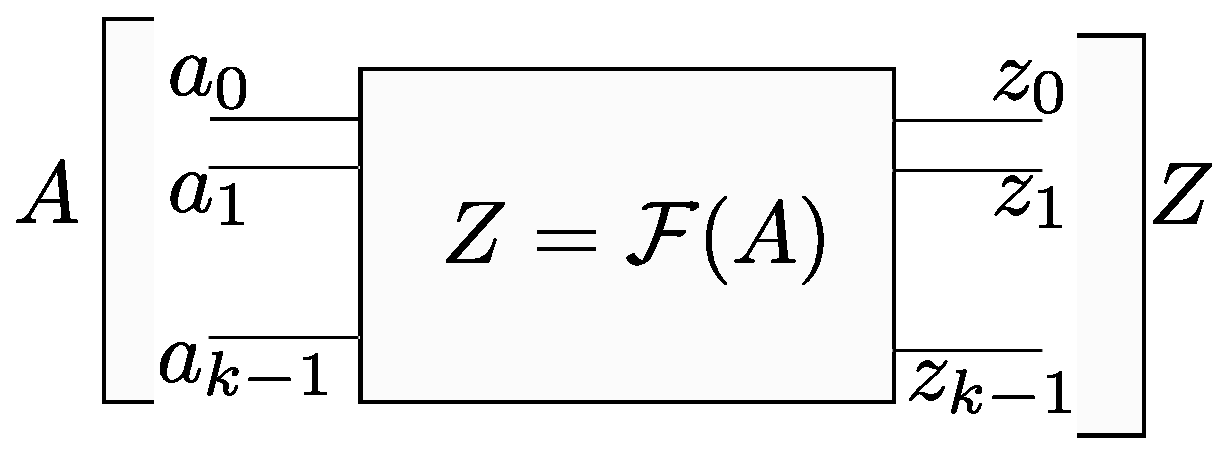
\includegraphics[scale=0.4]{interpolate.eps}
}
\begin{itemize}

\item Impose a lex term order $>$ on the polynomial ring such that \alert{circuit-variables including $a_0,\dots,a_{k-1},z_0,\dots,z_{k-1}> Z > A$}.
\item This elimination term order $>$: 
{\bf Abstraction Term Order} (ATO).

\item Compute a Gr\"obner basis $G$ of ideal $(J
+ J_0)$ using $>$
	\begin{itemize}
	\item $G$ will contain a polynomial of the form $Z + \F(A)$ ($Z = \F(A)$)
	\item $Z = \F(A)$ is a \alert{unique, canonical, polynomial}
  representation of $C$ over $\Fq$ 
	\end{itemize}
\end{itemize}
\end{frame}

%%%%%%%%%%%%%%%%%%%%%%%%%%%%%%%%%%%%%%%%%%%%%%%%%%%%
\begin{frame}{\large{Abstraction Term Order Example}}

\centerline{
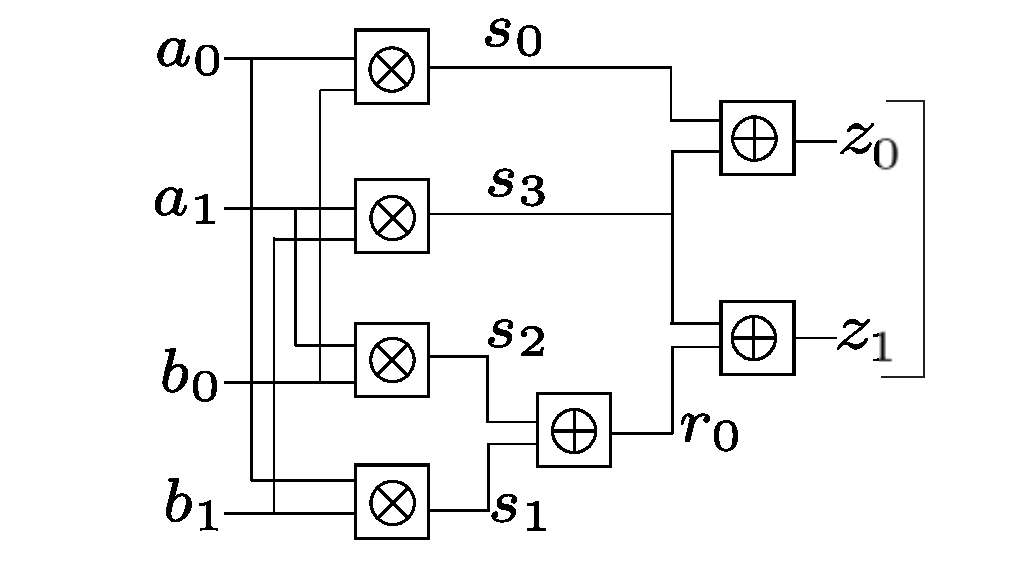
\includegraphics[scale=0.4]{2bitmult.eps}
}
%\vspace{-0.3in}
{\bf $(z_0 > z_1 > r_0 > s_0 > s_3 > s_1 > s_2 > a_0 > a_1 >  b_0 > b_1 > Z > A > B)$}
\begin{align*}
f_1: s_0+a_0 \cdot b_0; ~~f_2: s_1+a_0 \cdot b_1;  ~~f_3: s_2+a_1 \cdot b_0; ~~f_4: s_3+a_1 \cdot b_1  \nonumber \\
f_5: r_0+s_1 + s_2; ~~f_6: z_0+s_0 + s_3; ~~f_7: z_1+r_0+s_3; ~~f_8: a_0 + a_1 \alpha + A \nonumber \\ 
f_9: b_0 + b_1 \alpha + B; ~~f_{10}: z_0 + z_1 \alpha + Z \nonumber
\end{align*}
\vspace{-0.3in}
{\bf $J$ = $\langle f_1, \dots, f_{10} \rangle\ \ \ \ +\ \ \ \ J_0\ =\ \langle$vanishing poly $x^q-x\rangle$}
\end{frame}

%%%%%%%%%%%%%%%%%%%%%%%%%%%%%%%

%%%%%%%%%%%%%%%%%%%%%%%%%%%%%%%

\begin{frame}{\large{Abstraction Term Order Example}}

\centerline{
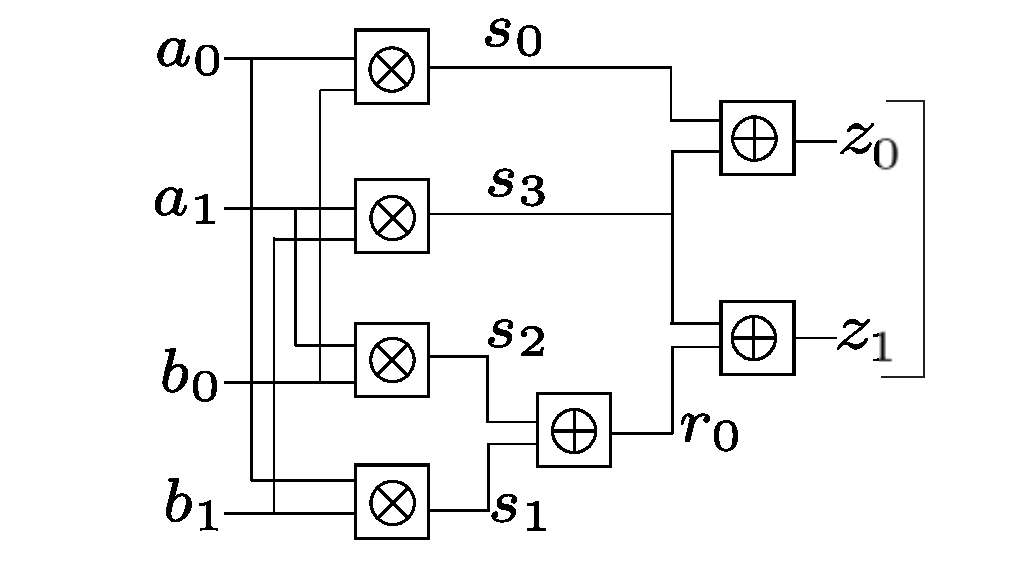
\includegraphics[scale=0.4]{2bitmult.eps}
}
%\vspace{-0.3in}
{\bf $(z_0 > z_1 > r_0 > s_0 > s_3 > s_1 > s_2 > a_0 > a_1 >  b_0 > b_1 > Z > A > B)$}

Compute the \Grobner basis, $G$, of \{$J + J_0$\} with respect to abstraction term ordering $>$.
$G$ = \{$g_1, \dots, g_{14}$\}
\begin{align*}
g_1: B^4+B; ~~g_2: b_0+b_1 \alpha + B; ~~g_3: a_0+a_1 \alpha + A; ~~g_4: A^4+A; \nonumber \\
g_5: s_0+s_1 \alpha + s_2 (\alpha + 1) + Z; ~~g_6: r_0+s_1+s_2; ~~g_7: z_1+r_0+s_3 \nonumber \\
g_7: z_0+z_1 \alpha +Z; ~~\alert{\bf g_9: Z+A*B} ; ~~g_{10}: b_1+B^2+B; ~~g_{11}: a_1+A^2+A \nonumber \\
g_{12}: s_3+a_1 b_1; ~~g_{13}: s_2+a_1 b_1 \alpha +a_1 B; ~~g_{14}: s_1+a_1 b_1 \alpha +b_1 A  \nonumber
\end{align*}

\end{frame}

%%%%%%%%%%%%%%%%%%%%%%%%%%%%%%



%%%%%%%%%%%%%%%%%%%%%%%%%%%%%%%%%%%%%%%%%%%%%%%%%%%%%%%%%%
\begin{frame}{\large{Verification of a sequential GF multiplier (Normal basis)}}
SPEC: $R = A_{init}\cdot B_{init} \pmod {P(\alpha)}$ after $k$ clock cycles
\hspace{-0.3in}\begin{figure}[hbt]
\centering{
%\begin{minipage}{12cm}
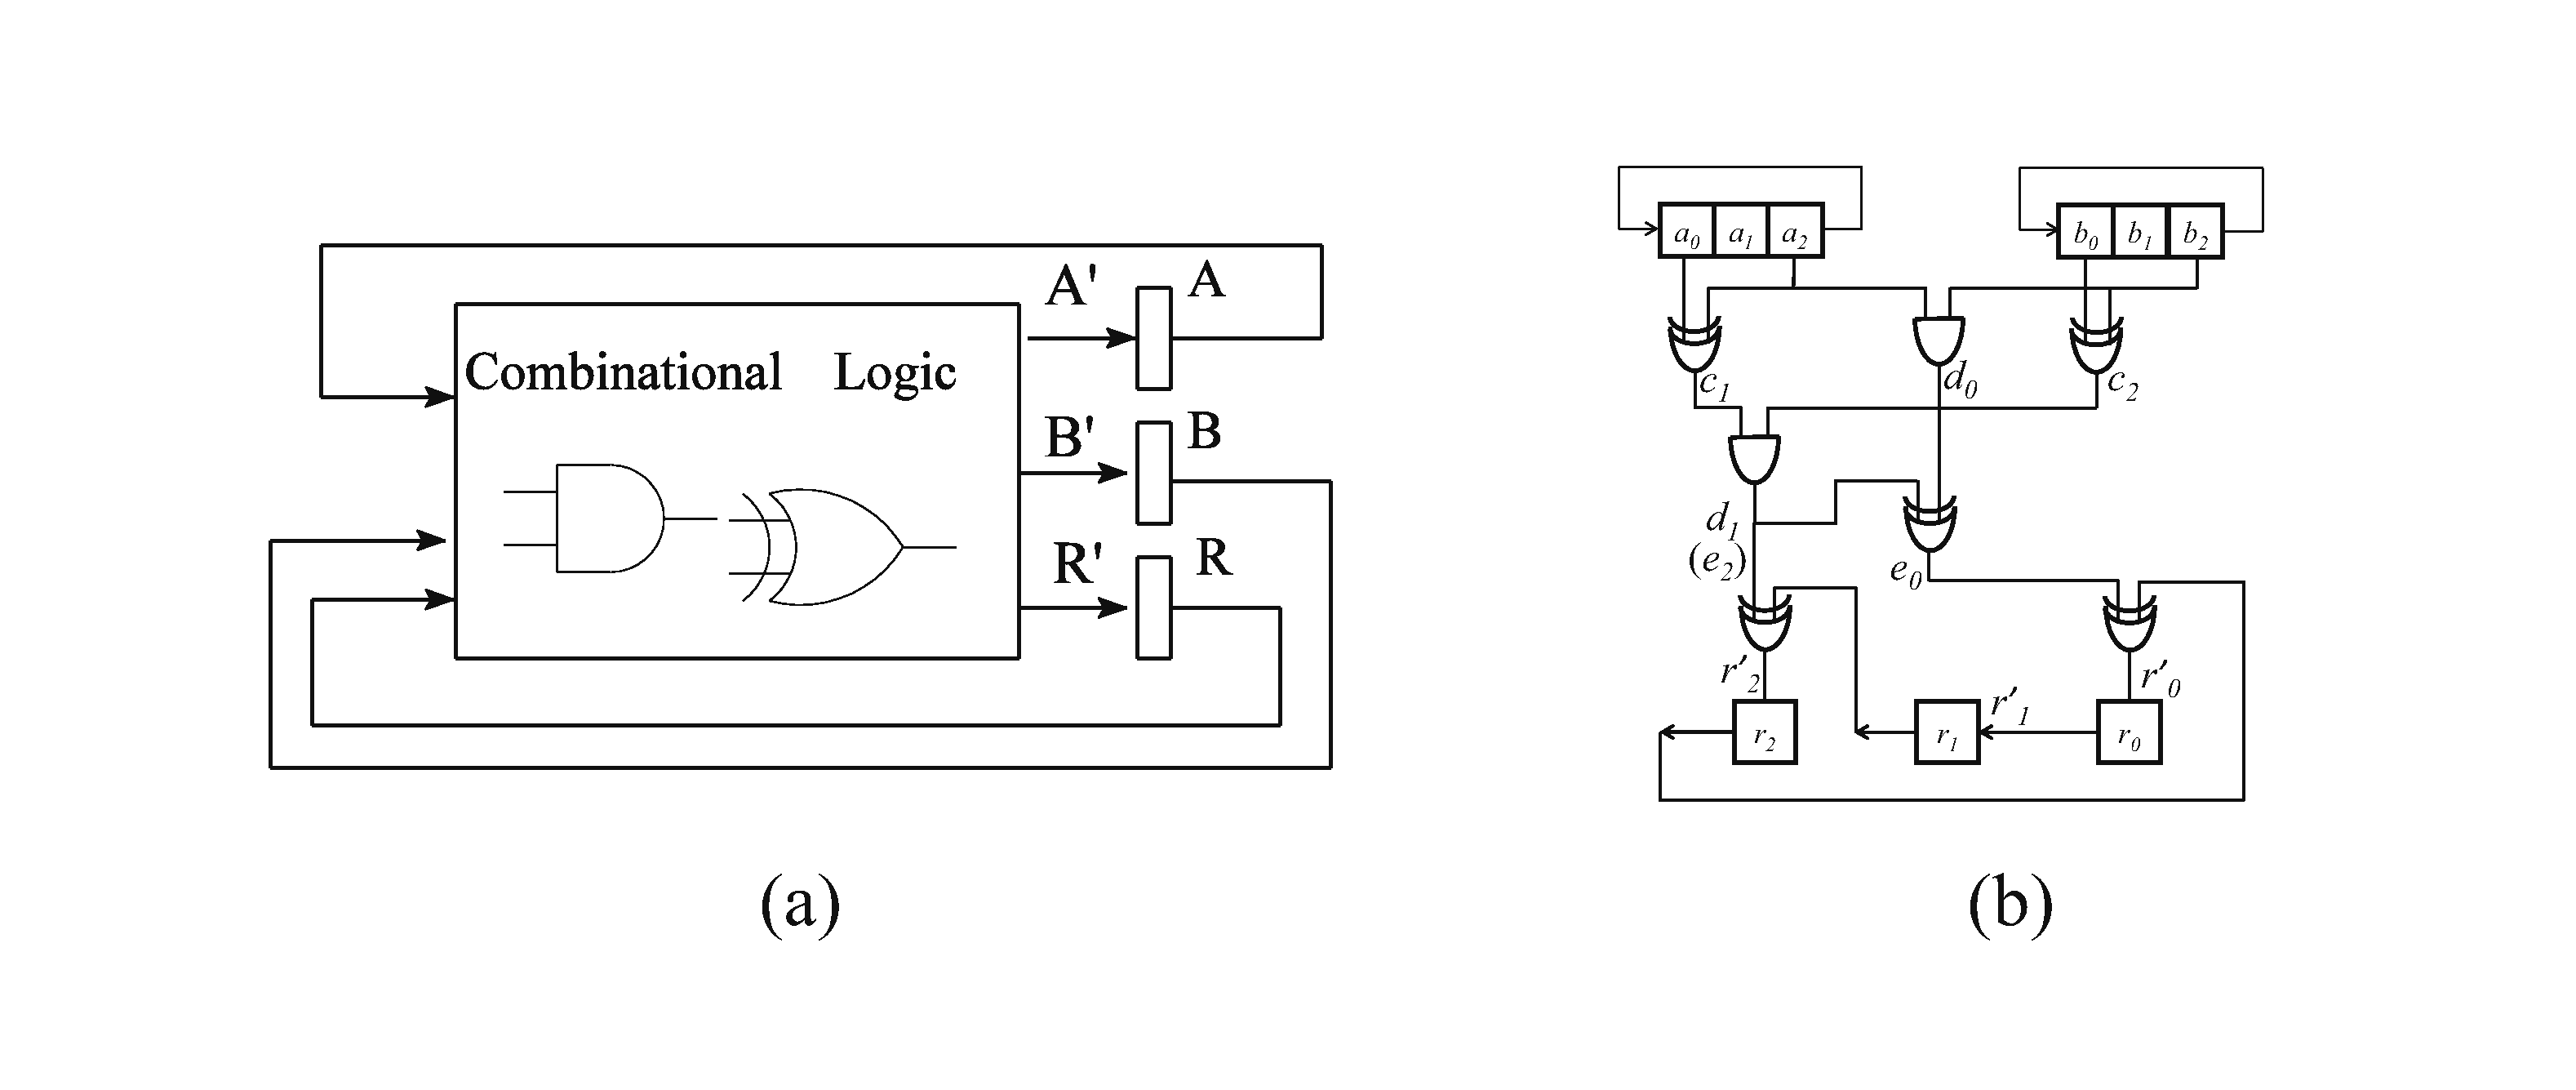
\includegraphics[width=5.5in]{./new_multi.eps}
% \vspace{-0.2in}
\caption{A 3-bit RH-SMPO and its Moore FSM model}
%\end{minipage}
\label{fig:RHmulti}}
\end{figure}
\end{frame}
%%%%%%%%%%%%%%%%%%%%%%%%%%%%%%%%%%%%%%%%%%%%%%%%%%%%%%%%%%%
% 
% \begin{frame}{\large{Galois field multiplication with normal basis}}
% \bi
% \item Let $R =
% \sum_{i=0}^{k-1} r_i \beta^{2^{i}}, ~A = \sum_{i=0}^{k-1} a_i
% \beta^{2^{i}}, ~B = \sum_{i=0}^{k-1} b_i \beta^{2^{i}}$, then 
% \[
% R = A\cdot B = (\sum_{i=0}^{k-1} a_i \beta^{2^{i}}) (\sum_{j=0}^{k-1}
% b_j \beta^{2^{j}})  =
% \sum_{i=0}^{k-1}\sum_{j=0}^{k-1}a_ib_j\beta^{2^i}\beta^{2^j}\nonumber 
% \]
% 
% \item Expressions $\beta^{2^i}\beta^{2^j}$ are called cross-product
% terms. Their normal basis representations are: 
% \begin{displaymath}
% \beta^{2^i}\beta^{2^j} =
% \sum_{n=0}^{k-1}\lambda_{ij}^{(n)}\beta^{2^n}, \ \ \lambda_{ij}^{(n)}
% \in \mathbb F_2. 
% \end{displaymath}
% \ei
% \end{frame}
% \begin{frame}{\large{Galois field multiplication with normal basis(2)}}
% \bi
% \item The expression for the
% $n^{th}$ digit of product $R = (r_0, \dots, r_n, \dots r_{k-1})$ is:
% \[
% r_n = \sum_{i=0}^{k-1}\sum_{j=0}^{k-1}\lambda_{ij}^{(n)}a_ib_j = A
% \cdot M_n \cdot B^T, ~~0 \leq n \leq k-1
% \]
% \item $M_n = (\lambda_{ij}^{(n)})$ is a binary $k \times k$ matrix over
% $\mathbb F_2$, and it is called the $\lambda$-matrix. 
% \item $\lambda$-matrix is \alert{unique} when $k$ and $\beta$ are given!
% \ei
% \end{frame}

%%%%%%%%%%%%%%%%%%%%%%%%%%%%%%%%%%%%%%%%%%%%%%%%%%%%%%%%%%%
\begin{frame}{\large{Basic algorithm to verify the function of sequential GF multipliers}}
\begin{algorithm}[H] % note [hbt] will fail in beamer
\SetAlgoNoLine
 \KwIn{Circuit polynomial ideal $J$, vanishing ideal $J_0$, initial state ideal $R (=0), \mathcal{G}(A_{init}), \mathcal{H}(B_{init})$} 

  $from_0(R,A,B) = \langle R, \mathcal{G}(A_{init}), \mathcal{H}(B_{init})\rangle$\;
  $i = 0$\;
  \Repeat{$i == k$}
  {
  	$i \gets i + 1$\;
	\alert{$G \gets$GB$( \langle J + J_0+ from_{i-1}(R,A,B) \rangle)$ with ATO}\;
	$to_i(R',A',B')\gets G\cap \mathbb F_{2^k}[R',A',B',R,A,B]$\;
	$from_i \gets to_i(\{R,A,B\}\setminus \{R',A',B'\})$\;
  }
\Return{$from_k(R_{final})$}
\caption {Abstraction via implicit unrolling for Sequential GF circuit verification}
\end{algorithm}
\end{frame}
%%%%%%%%%%%%%%%%%%%%%%%%%%%%%%%%%%%%%%%%%%%%%%%%%%%%%%%%%%
\begin{frame}{\large{Experiment on 3-bit RH-SMPO}}
\begin{figure}[hbt]
\centering{
%\begin{minipage}{12cm}
\includegraphics[width=1.5in]{./RH3.eps}
% \vspace{-0.2in}
%\caption{Gate-level circuit of 3-bit RH-SMPO}
%\end{minipage}
\label{fig:RHmulti}}
\end{figure}
\vspace{-0.2in}
\bi
\item The elimination ideal (first iteration):
\begin{align*}
J = &d_0+b_2\cdot a_2,
c_1+a_0+a_2,
c_2+b_0+b_2,
d_1+c_1\cdot c_2,\\
&e_0+d_0+d_1,
e_2+d_1,
r_0'+r_2+e_0,
r_1'+r_0,
r_2'+r_1+e_2,\\
&A+a_0\beta+a_1\beta^2+a_2\beta^4,
B+b_0\beta+b_1\beta^2+b_2\beta^4,\\
&R+r_0\beta+r_1\beta^2+r_2\beta^4,
R'+r_0'\beta+r_1'\beta^2+r_2'\beta^4;
\end{align*}
\ei
\end{frame}
%%%%%%%%%%%%%%%%%%%%%%%%%%%%%%%%%%%%%%%%%%%%%%%%%%%%%%%%%%%
\begin{frame}{\large{Experiment on 3-bit RH-SMPO(2)}}
\bi
\vspace{-3.45cm}
\item $J_0 = \langle x_i^2 - x_i, X^q - X\rangle$
\item $from_0 = \{R, A_{init}+a_0\beta+a_1\beta^2+a_2\beta^4,
B_{init}+b_0\beta+b_1\beta^2+b_2\beta^4\}$
\ei
\end{frame}
%%%%%%%%%%%%%%%%%%%%%%%%%%%%%%%%%%%%%%%%%%%%%%%%%%%%%%%%%%%
\begin{frame}{\large{Basic algorithm to verify the function of sequential GF multipliers}}
\begin{algorithm}[H] % note [hbt] will fail in beamer
\SetAlgoNoLine
 \KwIn{Circuit polynomial ideal $J$, vanishing ideal $J_0$, initial state ideal $R (=0), \mathcal{G}(A_{init}), \mathcal{H}(B_{init})$} 

  $from_0(R,A,B) = \langle R, \mathcal{G}(A_{init}), \mathcal{H}(B_{init})\rangle$\;
  $i = 0$\;
  \Repeat{$i == k$}
  {
  	$i \gets i + 1$\;
	$G \gets$GB$( \langle J + J_0+ from_{i-1}(R,A,B) \rangle)$ with ATO\;
	\alert{$to_i(R',A',B')\gets G\cap \mathbb F_{2^k}[R',A',B',R,A,B]$}\;
	\alert{$from_i \gets to_i(\{R,A,B\}\setminus \{R',A',B'\})$}\;
  }
\Return{$from_k(R_{final})$}
\caption {Abstraction via implicit unrolling for Sequential GF circuit verification}
\end{algorithm}
\end{frame}
%%%%%%%%%%%%%%%%%%%%%%%%%%%%%%%%%%%%%%%%%%%%%%%%%%%%%%%%%%%

\begin{frame}{\large{Experiment on 3-bit RH-SMPO(2)}}
\bi
\item $J_0 = \langle x_i^2 - x_i, X^q - X\rangle$
\item $from_0 = \{R, A_{init}+a_0\beta+a_1\beta^2+a_2\beta^4,
B_{init}+b_0\beta+b_1\beta^2+b_2\beta^4\}$ ($\beta = \alpha^3$)
\item $to_1 : 
R'+(\alpha^2) A_{init}^4 B_{init}^4+(\alpha^2+\alpha) A_{init}^4 B_{init}^2+(\alpha^2+\alpha) A_{init}^4 B_{init}+(\alpha^2+\alpha) A_{init}^2 B_{init}^4+(\alpha^2+\alpha+1) A_{init}^2 B_{init}^2+(\alpha^2) A_{init}^2 B_{init}+(\alpha^2+\alpha) A_{init} B_{init}^4+(\alpha^2) A_{init} B_{init}^2
$
\item $from_1 = \{
R'+(\alpha^2) A_{init}^4 B_{init}^4+(\alpha^2+\alpha) A_{init}^4 B_{init}^2+(\alpha^2+\alpha) A_{init}^4 B_{init}+(\alpha^2+\alpha) A_{init}^2 B_{init}^4+(\alpha^2+\alpha+1) A_{init}^2 B_{init}^2+(\alpha^2) A_{init}^2 B_{init}+(\alpha^2+\alpha) A_{init} B_{init}^4+(\alpha^2) A_{init} B_{init}^2
, A_{init}+a_2\alpha^3+a_0\alpha^6+a_1\alpha^{12},
B_{init}+b_2\alpha^3+b_0\alpha^6+b_1\alpha^{12}\}$
\item $\cdots$
\item After 3 iterations: $to_3 = \{ \alert{R'+A_{init}B_{init},}
~A_{init}+a_0'\alpha^3+a_1'\alpha^6+a_2'\alpha^{12},
~B_{init}+b_0'\alpha^3+b_1'\alpha^6+b_2'\alpha^{12}\}$
\ei
\end{frame}
%%%%%%%%%%%%%%%%%%%%%%%%%%%%%%%%%%%%%%%%%%%%%%%%%%%%%%%%%%%
\begin{frame}{\large{Refined Abstraction Term Ordering (RATO)[Pruss et al, {\it Abstraction using GB}, DAC'14]}}
\vspace{-0.2in}
\begin{columns}
\begin{column}{0.5\textwidth}
\bi
\item Computing GB: high computational complexity
\item Buchberger's algorithm simplified w/ special term order
	\item reverse-topological term order: \alert{only input variables left in remainder}

\ei
\end{column}
\begin{column}{0.5\textwidth}
\begin{figure}[hbt]
\centering{
%\begin{minipage}{12cm}
\includegraphics[width=1.5in]{./RH3.eps}
% \vspace{-0.2in}
%\caption{Gate-level circuit of 3-bit RH-SMPO}
%\end{minipage}
\label{fig:RHmulti}}
\end{figure}
\end{column}
\end{columns}
% \vspace{0.2in}
\begin{Example} 
Elimination ideal under RATO:
\vspace{-0.1in}
\begin{align*}
J = &d_0+b_2\cdot a_2,
c_1+a_0+a_2,
c_2+b_0+b_2,
d_1+c_1\cdot c_2,\\
&e_0+d_0+d_1,
e_2+d_1,
r_0'+r_2+e_0,
r_1'+r_0,
r_2'+r_1+e_2,\\
&a_0\alpha^3+a_1\alpha^6+a_2\alpha^{12}+A,
b_0\alpha^3+b_1\alpha^6+b_2\alpha^{12}+B,\\
&r_0\alpha^3+r_1\alpha^6+r_2\alpha^{12}+R,
r_0'\alpha^3+r_1'\alpha^6+r_2'\alpha^{12}+R';
\end{align*}
\end{Example}
\end{frame}

%%%%%%%%%%%%%%%%%%%%%%%%%%%%%%%%%%%%%%%%%%%%%%%%%%%%%%%%%%%
\begin{frame}{\large{Refined Abstraction Term Ordering (RATO) (2)}}
\begin{Example}
$$r_0'\alpha^3+r_1'\alpha^6+r_2'\alpha^{12}+R' \xrightarrow{J}_+$$
$(\alpha+1) r_1+r_2+\alpha b_1 a_1+(\alpha^2+\alpha) b_1 a_2+\alpha^2 b_1 A+(\alpha^2+\alpha) b_2 a_1+\alpha b_2 a_2+
(\alpha^2+\alpha+1) b_2 A+\alpha^2 a_1 B+(\alpha^2+\alpha+1) a_2 B+R'+(\alpha+1) R+(\alpha+1) A B$
\end{Example}
\bi
\item In [Pruss et al, {\it Abstraction using GB}, DAC'14], the authors did not address the problem when there are bit-level
input variables in the remainder.
\item Improve abstraction using RATO:
\ei
\begin{displaymath}
A = a_0\beta+a_1\beta^2+\cdots+a_{k-1}\beta^{2^{k-1}}
\end{displaymath}
\begin{displaymath}
\implies a_0 = \mathcal F_0(A), a_1 = \mathcal F_1(A), \dots
\end{displaymath}
\end{frame}
%%%%%%%%%%%%%%%%%%%%%%%%%%%%%%%%%%%%%%%%%%%%%%%%%%%%%%%%%%%
\begin{frame}{\large{Improve abstraction using RATO}}
\bi
\item Given word definition $A = a_0 \beta + a_1\beta^2 + \dots + a_{k-1}\beta^{2^{k-1}}$,
by squaring:
\begin{eqnarray}
A & = & a_0 \beta + a_1\beta^2 + \dots + a_{k-1}\beta^{2^{k-1}}\nonumber\\
A^2 & = & a_0 \beta^{2}+ a_1 \beta^{4} + \dots + a_{k-1}
\beta^{2\cdot 2^{k-1}} \nonumber\\
\vdots & \vdots& \vdots \nonumber\\
A^{2^{k-1}} & = & a_0 \beta^{2^{k-1}}  +  a_1 \beta^{2^{k-1}\cdot 2} +
\dots + a_{k-1}\beta^{2^{2(k-1)}} \nonumber
\end{eqnarray}
\item Write in matrix form:
\begin{displaymath}
\begin{pmatrix}
\beta & \beta^2 & \cdots & \beta^{2^{k-1}} \\
\beta^2 & \beta^4 & \cdots & \beta^{2^{k-1}\cdot 2} \\
\vdots & \vdots & \ddots & \vdots \\
\beta^{2^{k-1}} & \beta^{2^{k-1}\cdot 2} & \cdots & \beta^{2^{2(k-1)}}
\end{pmatrix}
\begin{pmatrix}
a_0\\
a_1\\
\vdots\\
a_{k-1}
\end{pmatrix}
=
\begin{pmatrix}
A\\
A^2\\
\vdots\\
A^{2^{k-1}}
\end{pmatrix}
\end{displaymath}
\ei
\end{frame}

%%%%%%%%%%%%%%%%%%%%%%%%%%%%%%%%%%%%%%%%%%%%%%%%%%%%%%%%%%%%
\begin{frame}{\large{Improve abstraction using RATO (2)}}
\begin{Example}
Solve system of equations using Gaussian elimination:
\begin{displaymath}
\begin{pmatrix}
\alpha^3 & \alpha^6 & \alpha^{12}\\
\alpha^6 & \alpha^{12} & \alpha^{24} \\
\alpha^{12} & \alpha^{24} & \alpha^{48}
\end{pmatrix}
\begin{pmatrix}
a_0\\
a_1\\
a_2
\end{pmatrix}
=
\begin{pmatrix}
A\\
A^2\\
A^4
\end{pmatrix}
\end{displaymath}
Results are:
\begin{displaymath}
\left\{
\begin{aligned}
&a_0 = (\alpha^2+\alpha+1)A^4+(\alpha^2+1)A^2+(\alpha+1)A \\
&a_1 = (\alpha+1) A^4+(\alpha^2+\alpha+1) A^2+(\alpha^2+1) A\\
&a_2 = (\alpha^2+1) A^4+(\alpha+1) A^2+(\alpha^2+\alpha+1) A
\end{aligned}
\right.
\end{displaymath}
Similarly replace $b_0,b_1,b_2,r_0,r_1,r_2$ with $B,R$
\end{Example}
\end{frame}

%%%%%%%%%%%%%%%%%%%%%%%%%%%%%%%%%%%%%%%%%%%%%%%%%%%%%%%%%%%%
\begin{frame}{\large{Final approach}}
\begin{algorithm}[H] % note [hbt] will fail in beamer
\SetAlgoNoLine
 \KwIn{Circuit polynomial ideal $J$, vanishing ideal $J_0$, initial state ideal $R (=0), \mathcal{G}(A_{init}), \mathcal{H}(B_{init})$} 

  $from_0(R,A,B) = \langle R, \mathcal{G}(A_{init}), \mathcal{H}(B_{init})\rangle$\;
  $i = 0$\;
  \Repeat{$i == k$}
  {
  	$i \gets i + 1$\;
	\alert{$f_o \xrightarrow{J + J_0+ from_{i-1}(R,A,B)}_+ f_r$ under RATO} \;
	\alert{$to_i(R',A',B')\gets f_r(\{R',A',B'\}\setminus\{r_0,\dots,r_{k-1},a_0,\dots,a_{k-1},b_0,\dots,b_{k-1}\}$}\;
	$from_i \gets to_i(\{R,A,B\}\setminus \{R',A',B'\})$\;
  }
\Return{$from_k(R_{final})$}
\caption {Abstraction via implicit unrolling for Sequential GF circuit verification}
\end{algorithm}
\end{frame}
%%%%%%%%%%%%%%%%%%%%%%%%%%%%%%%%%%%%%%%%%%%%%%%%%%%%%%%%%%%%

\begin{frame}{\large{Experiment results}}
\begin{table}[htb]
\centering
\caption{\small Run-time (seconds) for verification of bug-free and
  buggy RH-SMPO using our approach} 
\label{tbl:exp1}  
\begin{tabular}{|c||c|c|c|c|c|c|} 
\hline
Operand size $k$ & 33 & 51 & 65 & 81 & 89 & 99\\
\hline
\#variables & 4785 & 11424 & 18265 & 28512 & 34354 & 42372\\
\hline
\#polynomials & 3630 & 8721 & 13910 & 21789 & 26255 & 32373\\
\hline
\#terms & 13629 & 32793 & 52845 & 82539 & 99591 & 122958\\
\hline
\hline
Runtime(bug-free) & 112.6 & 1129 & 5243 & 20724 & 36096 & 67021\\
\hline
Runtime(buggy) & 112.7 & 1129 & 5256 & 20684 & 36120 & 66929\\
\hline
\end{tabular}
\end{table}
\bi
\item Experimented performed using SINGULAR
\item Note: Using conventional methods we cannot verify any multipliers with 23+ bits datapath
\ei
\end{frame}

%%%%%%%%%%%%%%%%%%%%%%%%%%%%%%%%%%%%%%%%%%%%%%%%%%%%%%%%%%

%%%%%%%%%%%%%%%%%%%%%%%%%%%%%%%%%%%%%%%%%%%%%%%%%%
\begin{frame}{\large{Conclusion}}
\bi
\item Succeed to verify large GF arithmetic circuits based on $k$-cycle unrolling
\item Provide a way to simplify GB computation
\item Has the potential to be applied to the verification of other sequential circuits
\ei
\vspace{4cm}
\textit{Singular code available: ece.utah.edu/$\sim$xiaojuns/codes.html}
\end{frame}


\end{document}
